\documentclass[a4paper,
  twoside, % to have to sided mode
  headlines=2.1 % number of lines in the heading, increase if you want more
  ]{scrartcl}
\usepackage[
  margin=2cm,
  includefoot,
  footskip=35pt,
  includeheadfoot,
  headsep=0.5cm,
]{geometry}

\usepackage{graphicx}
\usepackage{subcaption}
\usepackage{wrapfig}
\usepackage{float}
\usepackage{xcolor}
\usepackage{amsmath}

\author{Žiga Bradaš \\ \and Arjan Skok \\ \and Lukas Kneissl}
\title{Development of Intelligent Systems}
\subtitle{Delta Team Report}
\date{June 6, 2024}

\begin{document}

\maketitle

\newpage

\tableofcontents

\newpage

\section{Introduction}
This project’s work implements solving various tasks using a TurtleBot 4 in a simulated environment. The solution and simulation are based on ROS 2. The robot is a virtual version of the TurtleBot 4 and it operates in a pre-generated simulated world.
\\
The world is set up as a fenced area representing “a small renaissance town”. It includes the faces of several people, several paintings of Mona Lisa, colorful cylinders, pillars/boxes, hollow colorful cylinders hanging above, colorful cylinders drawn on boxes, and circular parking spots. The cylinders and rings are each in a single color. The cylinders represent “art galleries” and the rings mark parking spots. Some paintings of Mona Lisa are genuine and some are not. The ones that are not have anomalies on them. 
\\
The goal of the robot is to find the genuine Mona Lisa painting. There are several steps to achieving this goal. The robot has to find all the people in the city. It has to talk to each person to find out where a genuine Mona Lisa painting can be found. It should ask them about the colors that mark the correct parking position. Two of the people will respond with useful hints and the rest don’t know anything. The robot has to park in the right parking space. The location of which is signified by the appropriate hanging ring. When parked it has to scan a QR code on top of the nearest cylinder to obtain a photo of the genuine Mona Lisa. It then has to find the paintings of Mona Lisa, determine which one is genuine and point it out. 
\\
The robot has to explore the space and detect faces, paintings of Mona Lisa, cylinders and rings. It has to keep track their locations and attributes. It is important that it differentiates between faces of people and paintings of Mona Lisa as well as between the different colors of the cylinders and rings. The robot has to approach faces, cylinders and paintings of Mona Lisa. When approaching faces it has to engage in conversation with the person and extract information from their response. It must determine the location that overlaps in the useful answers and park there. To park it has to detect a parking spot on the ground under the appropriate ring and park in it. The parking spot is not exactly under the ring. When parked it must then go to the nearest cylinder and read the QR code on top of it. The QR code contains a link to a photo of the genuine Mona Lisa, which the robot must retrieve. When approaching a painting of Mona Lisa, it has to determine whether the painting is genuine or not based on the photo from the QR code and act accordingly. 
\\
The problem is simplified by the fact that photo of the Mona Lisa painting obtained from the QR code is always of the same genuine Mona Lisa. Thus, an anomaly detection method can be prepared in advance based on that. 


\newpage

\section{Methods}
\subsection{Navigation}
The navigation of the robot was divided into two sub tasks: building a map of the environment before the actual task begins and navigating on this map during the task.
\subsubsection{Building a map using SLAM}
Simultaneous Localization and Mapping (SLAM) is a key technology in mobile robotics that enables a robot to simultaneously create a map of its environment while also determining its own position within that map.\\
The difficulty here is that neither the motion models nor the sensor model can be perfect and therefore for both we have to rely on probabilistic methods to estimate, rather than calculate, how far the robot has moved with the last movement command or where a wall is most likely after it was detected by a sensor. What makes this problem even harder is that to update the so far built map from new sensor readings (like laser range finders) the robot must know its location on this map. At the same time, to determine its position on the already built map, the robot must know the map to interpret sensor readings correctly. It is a chicken-egg problem!\\
\\
To solve this problem, the 'Monte Carlo localization' is being used, also known as 'particle filter localization'. The Idea is that, instead of describing  the robots current position and the map with probability functions, we create many instances (particles). Each of those particles has his own map and his own robot position within that map.\\
Whenever the robot moves, some random error is added to the movement of each particle, to simulate one possible actual movement. The value of this error is determined by the used motion model. Usually it is much more likely that the robot ends up somewhere close to the targeted position than far away from it.\\
A simple implementation of this SLAM-method would use the sensor readings only to built the map, not to reposition the robot.\\
As the robot moves and scans, the reality of some of those particles will not add up. For example a particle that simulates a robot position very far from where the robot actually is on the map, or one that has built a very bad map, will eventually have a lot of measurements that don't fit the map and position that it has.\\
To use this fact, particles are being resampled. In simple therms: Particles that become very unlikely die out, while particles that seem very likely will be cloned. Each particle has a 'weight' that describes how likely it currently is. Scans that don't fit its state will reduce this weight while scans that fit it will increase the weight. Periodically particles with too little weight will be removed and particles with large weight will be duplicated. The higher the weight, the more clones are created of this particle. In total the number of particles stays the same. After this resampling, the weight of all particles is being reset to a default value.\\
What can be observed, after a while, is that the particles will form a cluster around the actual location of the robot and will contain more or less the actual map.\\
To get the final map we can for example combine the particles and build an weighted average map (particles with higher weight contribute more to the map than those with lower weight). Or we could simply pick the particle with the highest weight.\\
Since it is memory wise very costly to store an individual map for each particle, usually the number of particles is much lower than when we use the 'Monte Carlo localization' to localize the robot on a pre-built map. That brings us to the next topic: Navigating on a given map.


\subsubsection{Navigating on a given map}

\begin{wrapfigure}{r}{0.5\textwidth} %this figure will be at the right
    \centering
    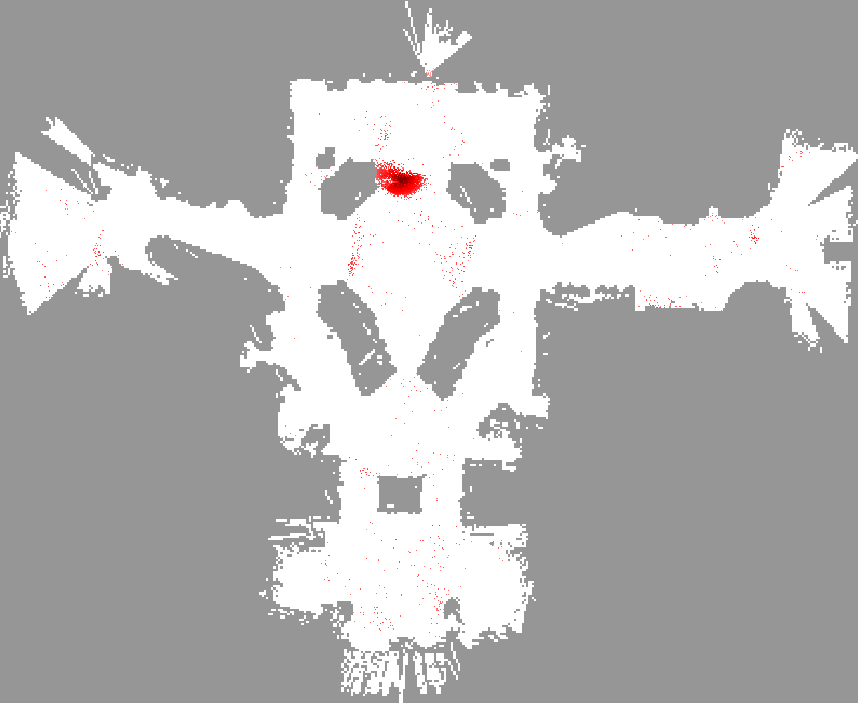
\includegraphics[width=0.4\textwidth]{monte_carlo_localization.png}
    \caption{'Monte Carlo localization' in action}
\end{wrapfigure}

This is a much simpler problem than described in the previous section, because now we know the map and we can assume it represents the reality precisely enough. So we only have to do localization on a given map to navigate safely on it.\\
Again the 'particle filter localization' is being used. This time however, each particles only simulates a possible robot position and not the whole map. So a lot more particles can be simulated. All particles share the given map, which is not being modified. Apart from that, the algorithm works very similar to what was described for the SLAM problem. Scans are being used to determine the likelihood for each particle and resampling makes sure that only particles that are good estimates of the actual position survive. To get a good estimate of the robots position we can calculate the weighted average position of all particles or pick the one with the highest likelihood (weight).

\subsection{Detection}
The task also required multiple different forms of object detections. Those objects were faces, 3D rings, cylinders, QR codes and anomalies on the painting.


\subsubsection{Face detection using YOLOv8}

\begin{wrapfigure}{r}{0.5\textwidth} %this figure will be at the right
    \centering
    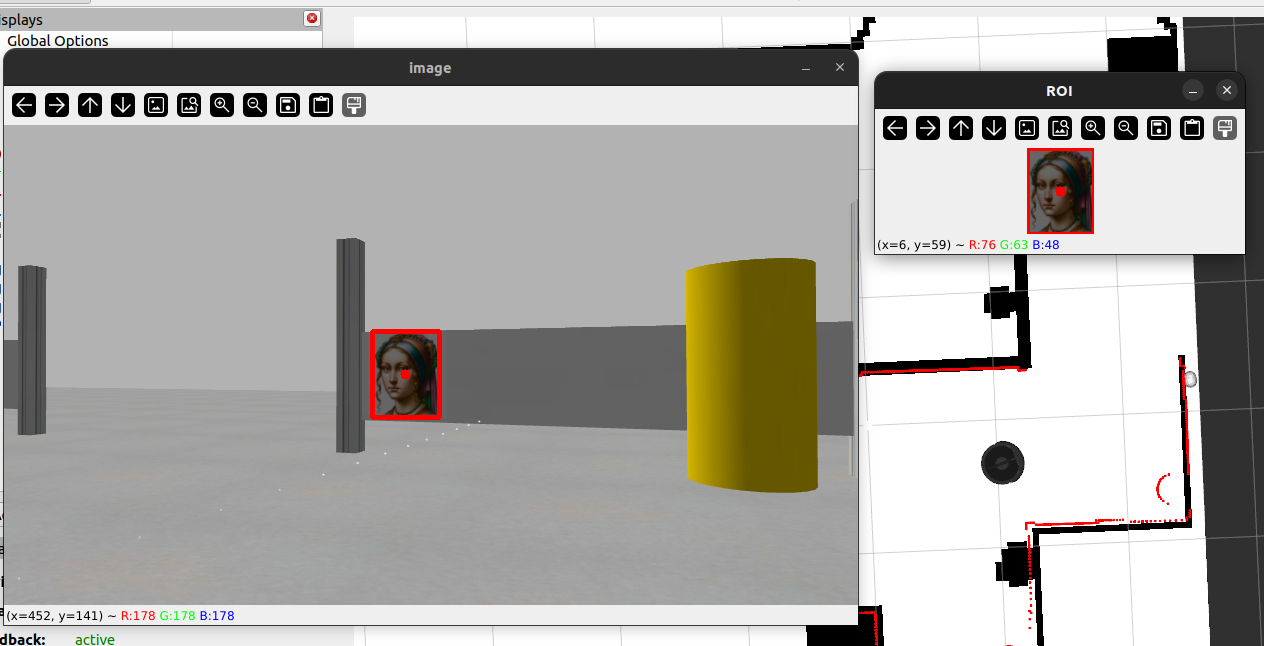
\includegraphics[width=0.5\textwidth]{YOLO.png}
    \caption{'YOLO detection'}
\end{wrapfigure}

For the task of face detection we used a model called YOLOv8. YOLO, which stands for "You Only Look Once" is a real time object detection model that uses convolutional neural networks. It's name comes from the fact that it's a single-stage object detector, that processes the image only once and returns bounding box probabilities for each region for the object we are detecting, which makes it much faster than two-stage object detectors. \\
The model can be trained for detecting multiple different types of objects. In our case our model is trained for detecting 80 different types of common objects, but we are only interested in faces. \\
The detection works in multiple stages. The input image, in or case a frame from the front camera, is first divided into cells using a grid and then passed through a CNN, which extracts the features from the image. Those are then passed through (2) fully connected layers, that transform those into an output vectors, which for each grid cell predict a set of bounding boxes and class probabilities. The bounding boxes are then filtered using non maxima suppression and the box with the highest probability is chosen. \\
In the end we get a set of bounding boxes with their class labels.



\subsubsection{Ring detection}
Detecting the hanging hollow rings works in a few stages. The image from the camera needs to be pre-processed first. Then rings can be detected. And finally, the detections need to be filtered to separate the actual desired rings from false detections and the unwanted rings. 
\\
The image from the RGB is binarized with adaptive thresholding. Binarization is performed on a grayscale version of the image. A threshold is determined for each pixel. The threshold value is the mean value in a square neighborhood of the pixel minus a constant. The grayscale image is transformed in to a binary image according to the formula: 
\\
\begin{equation*}
\text{dst}(x, y) = \begin{cases} 
\texttt{maxValue} & \text{if } \text{src}(x, y) > T(x, y) \\ 
0 & \text{otherwise} 
\end{cases}
\end{equation*}
\\
A border following algorithm is used to extract contours from the binary image.
\\
Ellipses are fitted to all the extracted contours by calculating an ellipse that best fits the set of points in a least-squares sense. The algorithm used for this is LIN: algebraic distance. 
\\
Two ellipses are required to constitute a ring. Their centers have to be approximately the same and their shapes very similar. One ellipse has to be larger than the other, that way the smaller ellipse is contained in the larger one. The larger ellipse corresponds to the outer edge of the ring and the smaller ellipse to the inner edge. Each possible pair of ellipses is checked to see if they form this combination. The pairs that do are candidates for ring detections. 
\\
Since our rings are hollow, their inner part is further away than their edge – the ring. The insides are usually so distant that they are perceived as out of range or infinitely far by the depth camera. We use this to determine whether our ring candidates are hollow. The robot’s course contains hollow rings hanging above and also rings drawn on the boxes. By keeping only the rings that are hollow, we get rid of the rings that are drawn on the boxes as those do not interest us as well as some false detections that might have slipped through the cracks until now. 
\\
To get the location of the ring we find a pixel on the actual ring, making sure that it is not in the hollow part. We choose the pixel closest to us in the depth camera. Transforming that with the point cloud gives us the approximate location of the ring. 
\\
To further eliminate false detections that have made it this far we also discard the rings bellow a certain height. The rings we are interested in are hanging above the course so they cannot appear in the bottom part of the camera frame. 
\\
The color of the ring is determined by taking the average color in the ring’s area, excluding the inner part. The average color is compared to a set of predetermined colors and the closest one is chosen as the color of the ring. 
\\
Newly detected rings are compared to a list of detected rings and their information. If a newly detected ring is too close to one of the already detected rings, it is considered a duplicate detection and is discarded. 



\subsubsection{Cylinder detection/segmentation}
For the detection of cylinders we use a method called RANSAC (Random Sample Consensus). RANSAC is an iterative algorithm that repeatedly selects a randomly selected subset of data and fits a model on it. After doing so it classifies all the other points of data as either inliers - points that agree to the model - or the outliers. It then repeats this process with a new randomly selected subsample every time, until it reach a predetermined number of iterations or an accurate enough model. The goal of the algorithm is to build such a model that maximizes the number of inliers.\\
RANSAC is a very robust algorithm, particularly useful when we have a data with a large number of outliers, which in our case it is. Even though RANSAC by itself randomly selects the inliers, so it isn't an optimal algorithm, we can still set some parameters that can improve the results. The main ones are the number of iterations, minimal number of inliers and the distance threshold, which determines how different data from the model still counts as inlier.\\
We are using 2 different specialized types of RANSAC. First we use a RANSAC to determine a main background plane of the detected pointcloud points. That type of RANSAC only needs 3 points to build a model (since it's a simple plane). After it finds the main plane, we can ditch all the inlier points, since we don't need them.\\
The second type we use is a RANSAC model for cylinder segmentation. This type also accepts the expected cylinder width range as the argument which is really helpful in our case where we know how big the cylinders are in advance. We only keep the inliers, that are supposed cylinders and ditch the rest of the points.\\
For the final part of the detection we use color and size recognition, which is a simple filtering based on rgb values (more on that in the third chapter).

\subsubsection{QR code detection}
For the QR code detection there are a few steps to be done (that an outside library does for us).\\
First we need to convert the image to greyscale and binarize it. Afterwards the three big squares should be recognized using a pattern recognition method. Those squares are necessary, so we know the orientation of the QR code. The perspective of the code can that way be corrected and transformed into a straight grid, no matter the original perspective and then a binary code can easily be extracted and translated into text.

\subsubsection{Anomaly detection}
The task of anomaly detection is to detect anomalies in Mona Lisa paintings. If a painting has an anomaly, then it is not genuine and vice-versa. We implemented anomaly detection by first capturing a dataset of images of the genuine Mona Lisa paintings and using them to train a model. The model used is an autoencoder and the classification in to genuine or not is done based on the reconstruction error when encoding and decoding an example. The idea is to have a photo of the genuine painting produce a low reproduction error and a photo of a painting with an anomaly produce a higher reproduction error. 
\\
First, we needed a dataset. We created one by creating a script that detects paintings of Mona Lisa in the camera’s image. It does this by detecting their frame. Images of these paintings are then saved. With this script running, we drove the robot around and looked at the genuine Mona Lisa paintings. We approached and looked at them in various different ways to create diverse example. We captured almost 900 images in this manner. There were some corrupted images among them and some images were of a painting with anomalies. In total there were about 50 of these and we eliminated them from the dataset. The remaining images form the raw dataset.
\\
Images in the raw dataset are of different dimensions as they are cropped out from the camera frame. They are also taken under different lighting conditions. We addressed these two concerns as well as the painting’s frame in the pre-processing of the dataset. 
\\
In the images from the raw dataset, the painting border is detected. The inside is kept and the rest set to black. The image is normalized to a range of [0, 1]. Each image is normalized individually. This equalizes the different brightness levels due to the difference in lighting conditions when capturing the images. The image is then padded with black pixels to make it square and afterwards resized to a desired resolution. The new resolution is lower than the previous. The result is a set of square images with black background, equal levels of brightness, and the painting content somewhere roughly in the center. We finally had a dataset that can be used with a machine learning model. 
\\
The model we used was an autoencoder. We trained it on the before mentioned set of processed images. 
To use the model, a frame from the camera of the robot is captured and processed in the same manner as the images in the dataset. The painting is cropped out, the frame and background are removed, the image is normalized, padded and resized. It is then encoded and decoded using the trained autoencoder. Afterwards, a reconstruction error is calculated between the original image and the reconstructed image. The reconstruction error is a mean of the differences squared.


\newpage

\section{Implementation and integration}

\subsection{Overview}
The communication between the nodes is almost completely done by publishing topic messages. We did not see a need to implement services or actions. Only the communication with the navigation is an exception where actions are used.\\
In the figure below is an overview of the nodes implemented for task 3.\\
\\
\textcolor{blue}{In blue:} Nodes that listen to relevant topics, process the information and publish new information. An example is the 'ring detection' node. It receives images from the front camera, tries to find rings in those images and publishes messages about the rings location and color if it finds one.\\
\\
\textcolor{green}{In green:} 'Servant' nodes get jobs from the 'mission control' node and execute them. They listen to job messages from the 'mission control' and continuously publish their status, which contains a JOB-ID and a JOB-STATUS. From those variables the 'mission control' stays informed if a job is still being processed or has finished already.\\
\\
\textcolor{red}{In red:} The 'mission control' node is the brain of the robot. It observes the mission status and makes decisions. If it wants one of the 'servant nodes' to execute a job, it will keep publishing messages, that contain a JOB-ID, until it catches a massage from a servant node, that contains this JOB-ID. That way it knows that the message was delivered. It keeps listening until it receives a massage with this JOB-ID and the JOB-STATUS 'finished'. Now it knows the task was executed and the mission can continue.

\newpage

\begin{figure}[H]
  \centering
  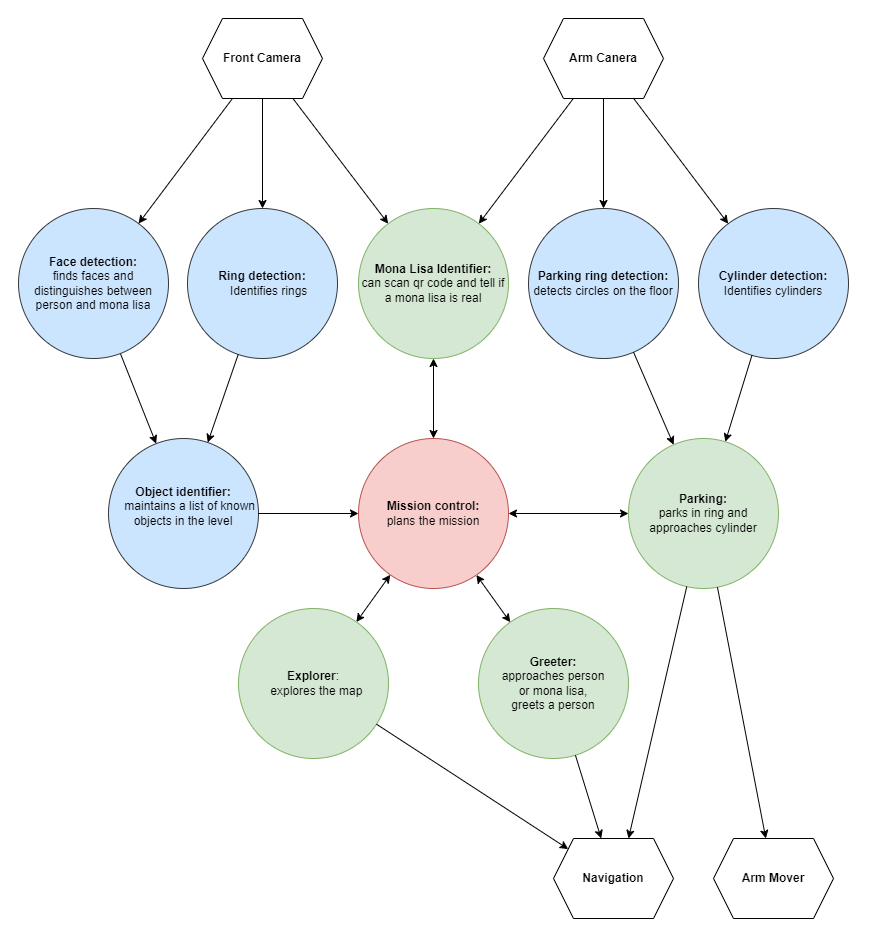
\includegraphics[scale=1.0]{node_overview.png}
  \caption{Node overview}   
\end{figure}

The next sections will explain the most important nodes in more detail.\\

\subsection{The 'Mission Control' Node}

\begin{figure}[H]
  \centering
  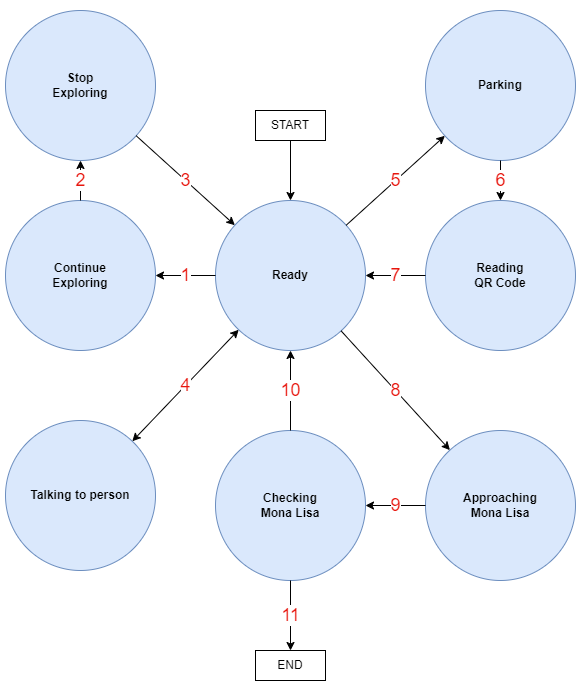
\includegraphics[scale=1.0]{mission_control.png}
  \caption{States of the 'mission control' node}   
\end{figure}

This node is something like the robots brain. It is built like a state machine and depending on the circumstances it will change to another state. In the beginning it is in the state 'ready'.\\
It follows a list of the possible transitions:\\
\\
1: If there is nothing else to do, the robot will continue exploring.\\
\\
2: The robot stops exploring, if:\\
- It still needs to find out the color of the ring and it knows a person it has not talked to yet\\
- It knows the color of the ring and has found the ring but not parked yet.\\
- It has parked (and scanned qr code) already and knows a mona lisa it has not checked yet.\\
\\
3: When the robot has successfully stopped exploring it will return to the status 'ready'.\\
\\
4: If the robot still needs to find out the color of the ring and it knows a person it has not talked to yet, it will go into status 'talk to person'. Once it is done it will return to status 'ready'.\\
\\
5: The robot knows the color of the ring and has found the ring but not parked yet.\\
\\
6: The parking is complete. This also involves approaching the cylinder.\\
\\
7: The qr code was successfully read.\\
\\
8: The robot has parked (and scanned qr code) already and knows a mona lisa it has not checked yet.\\
\\
9: The mona lisa was approached and is now visible by the front camera.\\
\\
10. The checked mona lisa was fake.\\
\\
11. The checked mona lisa was real.

\subsection{Exploration}
We used hard coded positions on the map and added to each position a start and an end rotation. The navigation was then first ordered to approach the next position, looking towards the start rotation and rotate then to the end rotation. That way the robot did not have to spin 360 degree at each point but could explore a bit more efficient.\\
The communication with the navigation was encapsulated in its own class, which every node that had to talk to the navigation could use.\\
\subsection{Parking}
The parking node receives the coordinates where it should park from the mission control in its job message. It first sets a navigation goal to this position and moves the arm in the correct position, facing towards the floor. The parking node then listens to the 'parking ring detection' node until a circle on the ground is detected (and the robot is already close enough to the ordered parking destination). If that happens before the navigation reached its goal, the navigation is stopped. If it doesn't happen, a simple search algorithm tries to find the circle in the area (basically: move forward 0.1 meters, turn 360 degree. repeat until you find the ring).\\
The robot then turns towards the center of the ring and moves half the distance to the rings center. It repeats this until it is close enough (less then 5 cm) to the center. Because the node remembers the world position where the ring was last spotted it can continue the approach even if the ring is no more visible on the camera.\\
Once the parking is complete, the navigation is used to rotate the robot, until a cylinder is spotted within a certain range. The robot then approaches that cylinder by rotation towards it and moving forward a bit, until it is close enough for the arm camera to read the qr code.

\subsection{Navigation}
This is the navigation node of ROS 2. It provides action servers for different actions. The ones we used were:\\
\\
\textbf{NavigateToPose:} The robot navigates to a given world position.\\
\textbf{Spin:} The robot spins by the given degree.\\
\textbf{DriveOnHeading:} This can be used to move the robot forward by a given value.\\
\\
To communicate with the navigation, the necessary code was encapsulated in a class which all nodes that needed to use the navigation could use.

\subsection{Greeter}
The greeter node receives a job via a topic subscription. Once it receives a job it checks if it is already executing a job or if it has already received the same job and if neither is true, it starts executing the job and publishes this as a status. The jobs it receives are to greet a person. The job message contains the location of the person and some other attributes.
\\
It first executes a move to the position where it will greet a person. The move is done with the help of a robot controller. While moving to the position, it publishes a marker indicating the greeter navigation goal. 
\\
When the robot is in position, it publishes a marker indicating a talk with the person. Then it plays an audible greeting with the help of a text-to-speech library. It listens for a response, capturing the audio from the microphone. The audio capture continues until the person stops speaking. When the capture is finished, the node performs speech recognition on the captured audio clip. The recognition is done with Google’s Web Speech API. There is also a fallback option of using the Sphinx service instead, should Google’s API be unavailable. 
\\
The recognition returns text from which colors are extracted. The response differs based on the number of unique colors extracted. The robot reports the number of extracted colors and their names. If one or more colors are extracted, it saves the first two colors (of only one was extracted, the second is a value signifying no color) to dedicated attributes. 
\\
After this, the node changes its status to indicate it is no longer executing a job and publishes it. Along with this indication, the colors are also published. The topics that require them will be able to get them from this message. 


\subsection{Face detection}
The face detection node is periodically recieving front camera rgb images (frames). First we perform face detection using YOLOv8, which gets us a bounding box around the detected face. \\
Because YOLO detects both real people and Mona Lisas we need to somehow differentiate between them. For that purpose we use histogram comparison method, which takes RGB values from the image and creates a histogram representation. Because we know that we need to separate Mona Lisa from people, we can upload the image of it into the node, and create a template histogram from it. That way we can compare the histogram from detected person (using the extracted pixels inside the bounding box rectangle) to the histogram of Mona Lisa and calculate the similarity value. If similarity is high enough it means that the detected "person" is Mona Lisa, otherwise it's a person. \\
Because of lighting changes and lower resolution we left a buffer zone of values in between for safety, where the detected figure is neither person nor the painting. \\
After the differentiation is done, we publish a marker on the map using tf2 pointcloud transformation, either a white or a red one, depending if it's a person or Mona Lisa.

\subsection{Ring detection}
The ring detection node is subscribed to the camera images and point cloud. The RGB image, depth image and point cloud each have their own callback function. These callback functions are assigned to their respective subscriptions and are called on the data.
\\
The RGB image is first converted to grayscale. Adaptive thresholding is applied as described in the methods. The resulting binary image is given to the contour-finding algorithm. The returned contours are iterated over and ellipses are fitted if the contour is of sufficient enough size. A double loop iterates over these ellipses. The outer loop iterates over all the ellipses and the inner loop iterates over the remainder of the ellipses from the one that is the current ellipse in the outer loop. This way all unique pairs of ellipses are iterated over. For each pair, the distance between their centers and the angle difference are calculated. If the centers aren’t close enough or the angle difference is too big, the pair is skipped. If not, it is determined which is the larger and which is the smaller ellipse. The two ellipses are saved to the list of ring candidates as a pair of a smaller and a larger ellipse.
\\
A separate loop iterates over the list of candidates for rings. A mask that lets through the ring pixels and covers the rest is created for the image. The average color of the ring area is calculated using this mask. The color is assigned a name based on the values of color channels. A ring object holding the information about the ring is created. It holds the ring id, center point, corners, masks of the ring and both ellipses, and the color value and name. The object is appended to a list of ring candidates in the node object. 
\\
For each ring from the list of ring candidates in the node object, the depth image is masked with the inner ellipse mask. The presence of infinite values in this area indicates that the ring is hollow and attribute in the ring’s ring object is set to true or false accordingly.
\\
For each ring from the list of ring candidates that is hollow, a point on the ring (on the edge and not in the inner, hollow, part) is determined. The closest point in the area is taken for this. This point is transformed with the point cloud to get the location of the ring. If the transformation is unsuccessful, the ring candidate is dropped. The ring candidate with this new location information and all previous information is then compared to a list of confirmed detected rings, also stored in the node object. If the new ring is not too close to any of the existing detections, it is added to the list as a new detected ring. In this case, a marker is also published indicating the ring location and color. 
\\
The image operations are done with the OpenCV library.


\subsection{Cylinder detection}
The cylinder detection node is periodically recieving front camera pointcloud. First we extract the planar inliers using RANSAC based segmentation for plane detection. On the inliers we then perform another RANSAC, this time a segmentation for clylinder detection.\\
After that we are left with only the pointcloud detections of objects similar to cylindrical shape. But the detection is still inaccurate with many false positives.\\
To solve that we can use the color properties of the cylinders, which are really distinct bright colors. Because the pointcloud points also carry the RGB information, the process is easy. First we calculate the average RGB values of each of remaining pointcloud object. If the absolute difference between the channels is small enough (the detected object is greyish), we ditch those detections. We also check, if the pointcloud size is large enough, since the cylinders on the map are quite big. This and the maximum height on which cylinder can be detected, solves all of our problems. What's left is a really robust cylinder detector that publishes the cylinder locations as markers.

\subsection{Parking ring detection}
This node is a simplified version of the ring detector that uses the arm camera. It is detecting all circles on the map using the contour detection and fitting elipses on those contours, no matter if they are on the ground, on the wall, or floating. Since its output is only used during the parking process, we found it works well enough without additional tweaking.\\
Once the robot starts parking, the arm points the camera to the ground, a bit in front of the robot. When the detector sees a ring it publishes the center coordinates as a marker. It continues to do so, until the robot drives so far ahead during the parking that the ring is not fully visible anymore.

\subsection{Object identifier}
Our detectors send the detection markers every time they detect an appropriate object, no matter if they have already done so in the previous frame or not. Because we want to know if the object has already been detected or not, we need to filter out the detections somehow. For that end we implemented the object identifier node.\\
We have two separate identifiers: one for the faces and one for cylinders, but they both work by the same principle. The identifier is subscribed to the marker topic of the face/cylinder detector. Once it gets a new marker, it checks, if there is already a known object on that location. If it's not, it adds it to the list that keeps all the known objects. We keep track of the location and in the case of the cylinders color. If there is already a face/Mona Lisa or a cylinder in a determined radius around the newly seen one, it throws it away.\\
Since face/Mona Lisa separator sometimes returned false positives (eg. it said that Mona Lisa is a face, if it saw just the part of it), we implemented an additional failsafe. For the face to be counted, there need to be 10 detections in the same place, and if even one of those is marked as Mona Lisa, it means that the detected face is actually Mona Lisa. That way we always get an accurate identity in the end.\\
The node is periodically publishing a list of know objects to the mission control.

\subsection{Mona Lisa identifier}
This node serves two separate purposes.\\
The first one is QR code detection. If the arm camera detects a QR code (after it got the order to start doing so from the mission control) it reads it and then checks if the data it got contains a link to a PNG file. If it does, it downloads the image into the node and displays it in the popup window.
The second purpose is checking if the detected Mona Lisa is a real one or a fake. 
\\
The second one is classification of Mona Lisa paintings in to genuine or not genuine through anomaly detection. The node object contains the autoencoder model, loaded on object initialization. When the node is called to perform Mona Lisa classification, a flag in the object node is set. This flag is checked in the RGB callback. If true (meaning: do Mona Lisa classification), it takes the image of the painting and prepares it using the appropriate functions. These are the same functions used in the preparation of training data for the model. The prepared image is then passed through the model. The model is an autoencoder model from TensorFlow Keras. Encode and decode operations are performed to produce a reproduction of the image. The original and the reproduction are then compared to calculate an error. The images are subtracted and squared pixel-wise. Afterwards, the mean error is taken as the reproduction error. Based on a threshold, a flag is set to either true or false, indicating whether or not the painting is genuine. The robot reports the result and publishes the status. The status publish includes the flag indicating whether the painting is genuine. 

\subsection{Arm mover}
The node serves as the operator of the robotic arm. It is subscribed to a topic, where we can publish the orders for the arm movement and based on it then sends the orders to an action server that controls the arm's joints. We can either send it one of four predefined arm positions, or send the joint values ourselves.

\subsection{Anomaly detection}

While not a node or part of the final implementation, we feel that the process behind the anomaly detection model was significant enough to warrant a section here.
\\
We made a copy of the face detection node and modified it to perform rectangle detection in a similar fashion as ellipse detection in the ring detection node. 
\\
It transforms the image to grayscale and applies adaptive thresholding to produce a binary image. Then it finds contours in the binary image. It iterates over the contours performs polygon approximation using the Douglas-Peucker algorithm. The approximations with 4 corners are added to a list of rectangle candidates. Then it finds pairs of rectangles that are close enough and similar in size and saves the larger one to a list of rectangles. The larger and smaller rectangle in such a pair are the outer and inner border of the painting frame. 
\\
The list of rectangles, selected in this way, is then iterated over and the section of the image is cut out. The new, cut out, image is then saved to a file. A list of hashes already saved images is kept and checked against to avoid saving duplicates of the same image. 
\\
We then processed these captured images to form a suitable dataset. 
\\
The image is thresholded based on the color of the frame, resulting in a painting frame mask. Contours are then fitted to the mask. The area inside the frame is kept. The area of the frame and the area outside of the frame are turned to black. The image is then normalized to a range of [0, 1]. Each image is normalized separately. 
\begin{figure}[H]
  \centering
  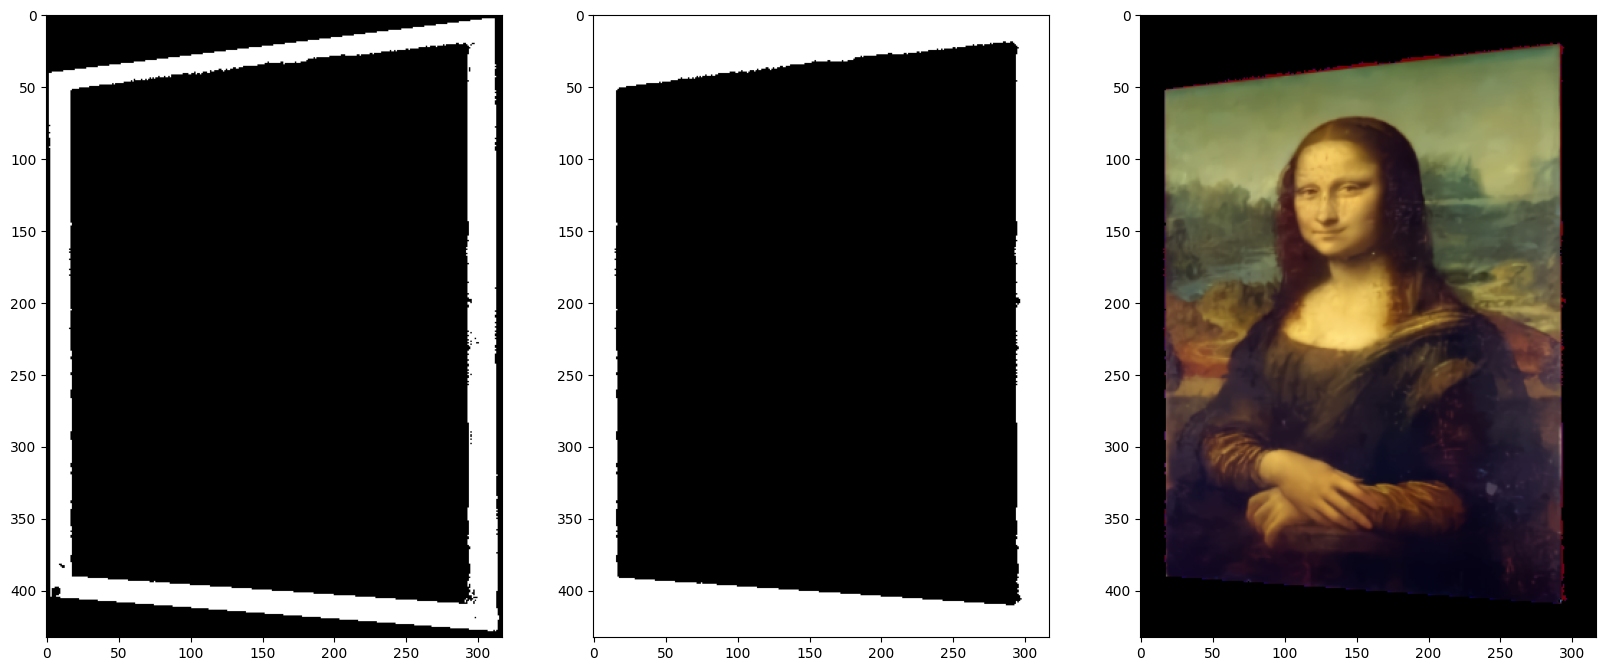
\includegraphics[scale=0.4]{dataset preparation 1.png}
  \caption{A visualization of the image pre-processing steps (from left to right: frame mask, painting mask, resulting extracted painting area)}   
\end{figure}

\noindent The image is then padded with black pixels to make it square. Afterwards it is resized to a desired resolution. In this case, this means downscaling as raw captures are of higher resolution than the images that go in to the model. The size chosen was 128 by 128 pixels.
\\
The result is saved to a new file. This is done for all the images in set.
\\
\\
The model is an autoencoder. The encoder uses ReLU activation and the decoder sigmoid activation. It is trained on the set of processed images. The dataset is split randomly in to a larger training portion and smaller test portion. We found that a latent dimension of 128 and 30 epochs of training produce a satisfactory result. The training uses MSE as the loss function. The model is saved to a file.
\begin{figure}[H]
  \centering
  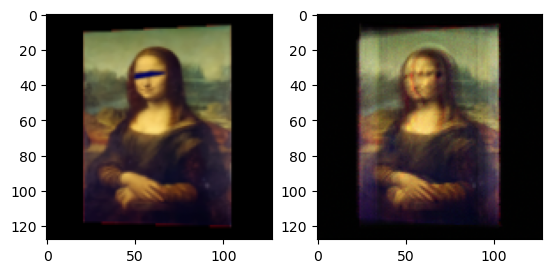
\includegraphics[scale=0.76]{model img pass 1.png}
  \caption{An image with an anomaly, passed through the model (original processed image and reconstruction}   
\end{figure}
The reconstruction error is calculated by taking the mean of pixel-wise squared subtraction between the images.
\\
By passing an example of an image with an anomaly through the model, we can see the reconstruction error:
\begin{figure}[H]
  \centering
  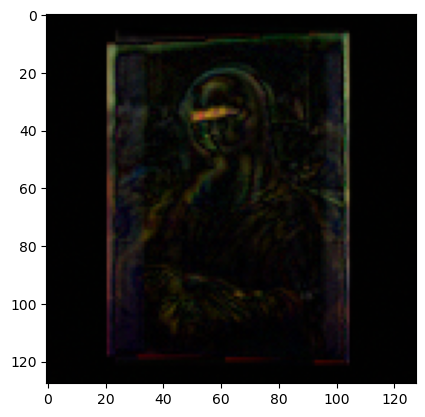
\includegraphics[scale=0.54]{model img recon diff 1.png}
  \caption{Visualized reconstruction error}   
\end{figure}


\newpage

\section{Results}
The result is a working (virtual) robot, that can solve most of the original task. 
\\
The robot drives around the space. It detects faces, paintings, cylinders and rings. When it detects cylinders and rings, it notes their attributes like location and color, and publishes markers. When it detects a painting, it takes note of its location and publishes a marker. When it detects a person, it approaches it and has a conversation. From the conversation, it extracts colors and notes them down. When it receives enough hints about colors to determine the right parking spot, it drives to it and executes a parking maneuver. Then it approaches the corresponding cylinder and reads the QR code. From the QR code, it gathers the link and downloads the image of Mona Lisa. Then it approaches Mona Lisa images and runs classification on them until it discovers a genuine one. It would point out a genuine one, perform a wave with the arm, and stop its mission.
\\
The ring detection is not as robust as we would like. It works most of the time, but sometimes it still acts up. 
\\
The anomaly detection and Mona Lisa classification work well offline (outside of ROS). However, in the implementation with ROS, there are some issues with the camera image and the image preparation in Mona Lisa identifier node, that cause it to crash often. 


\newpage

\section{Division of work}
\textbf{Žiga Bradaš: (33.3 \%)}\\
- Mona Lisa anomaly detection (including data capture, dataset preparation, model training)\\
- Robot conversation with user (text to speech and speech to text)\\
- Git administration (for example saving code from lab laptops to repository after work)\\
- Ring detection\\
\\
\textbf{Arjan Skok: (33.3 \%)}\\
- Cylinder detection\\
- Adapting ring detection to detect parking rings\\
- Person / Mona Lisa separation\\
- QR code scan and saving Mona Lisa image\\
- Work on object identifier\\
\\
\textbf{Lukas Kneissl: (33.3 \%)}\\
- Parking and cylinder approach\\
- Communication with ROS2 navigation\\
- Mission logic (mission control node)\\
- Integration of nodes into the project and communication between the nodes\\
- First version of object identifier\\
- Exploration
\\
\\
The overall idea/design and structure of the system and this final report are a group effort.

\newpage

\section{Conclusion}
In conclusion, most of the task solutions work well. The two problematic ones could use some additional polishing and debugging. We got them to work well in a development environment, but ran in to more issues than expected when carrying them over to ROS and the final implementation. 
\\
During the project we also ran in to countless issues with ROS itself and even more so the Gazebo simulation. 
\\
We learned some new approaches and methods in machine learning and robotics. We gained a lot of experience in putting various methods and approaches to use in practice and discovered the nuances that come with a more real-world-like system and environment. There were also some important lessons on robustness.


\end{document}